The analog mother board is instrumented with eight 16-channel FE ASICs,
eight 16-channel ADC ASICs, LV power regulators, and input-signal protection circuits.
The 16-channel FE ASIC provides amplification and pulse shaping.
The 16-channel ADC ASIC comprises 12-bit digitizers performaning at speeds up to 2 MS/s, local buffering,
and an 8:1 MUX stage with two pairs of serial readout lines in parallel. The 2017 ProtoDUNE Single Phase (ProtoDUNE-SP) version of the FEMB is shown in Figure~\ref{fig:femb}.

\begin{dunefigure}
[The complete FEMB assembly as used in the ProtoDUNE-SP detector. The cable shown is the high-speed data, clock, and control cable.]
{fig:femb}
{The complete FEMB assembly as used in the ProtoDUNE-SP detector. The cable shown is the high-speed data, clock, and control cable.}
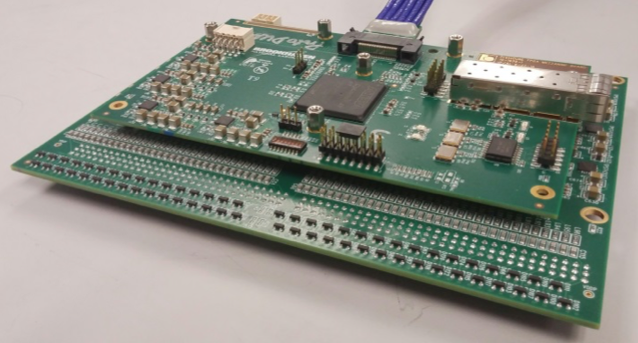
\includegraphics[width=0.6\linewidth]{tpcelec-femb.png}
\end{dunefigure}
